\documentclass[a4paper,11pt]{beamer}
\usepackage[utf8]{inputenc}
\usepackage{lmodern}
\usepackage{caption}
\usepackage{subcaption}
% Thème Darmstadt
\usetheme{Darmstadt}
\usepackage{graphicx}
\usepackage{caption}
\usepackage{ragged2e}
\usepackage{listings}
\usepackage{color}
\usepackage{gitdags}
\usepackage{fontawesome, wasysym}
%\captionsetup[figure]{labelformat=empty}

\setbeamertemplate{navigation symbols}{} 
\setbeamertemplate{footline} 
{  
	\begin{beamercolorbox}[ht=2.5ex,dp=1.125ex,%
      leftskip=.3cm,rightskip=.3cm plus1fil]{title in head/foot}%
      {\usebeamerfont{title in head/foot}\insertshorttitle} \hfill    
      \insertframenumber / \inserttotalframenumber%
    \end{beamercolorbox}%
%     \begin{beamercolorbox}[colsep=1.5pt]{lower separation line foot}
%     \end{beamercolorbox} 
}

% Informations sur la présentation
\title{Gestion de code avec Git (FIEC30EM)\\ - Le projet -}
\author{frank.buloup@univ-amu.fr} 
\institute{Aix Marseille Université\\Faculté des Sciences du Sport\\Master 2 IEAP - Facteurs Humains}
\date{}

\newcounter{exampleBlockCounter}
\setcounter{exampleBlockCounter}{1} 

\definecolor{comment}{rgb}{0.12, 0.38, 0.18 } %adjusted, in Eclipse: {0.25, 0.42, 0.30 } = #3F6A4D
\definecolor{keyword}{rgb}{0.37, 0.08, 0.25}  % #5F1441
\definecolor{string}{rgb}{0.06, 0.10, 0.98} % 

\lstset{
language=Python,
frame=single,
frameround=tttt,
rulesepcolor=\color{black},
showspaces=false,showtabs=false,tabsize=2,
numberstyle=\tiny,numbers=left,
stringstyle=\color{string},
keywordstyle = \color{keyword}\bfseries,
commentstyle=\color{comment}\itshape,
basicstyle=\ttfamily\footnotesize,
breaklines=true,
captionpos=b
}

%\includeonlyframes{current}

\begin{document}

% Première diapositive : Titre
\begin{frame}[plain]
    \titlepage
    \center{
\includegraphics[scale=0.75]{images/by-nc-sa.eps}}
 	\vspace{0.5cm}

	
\includegraphics[scale=0.6]{images/LogoAMU.png}\hspace*{2cm}
	
\includegraphics[scale=0.35]{images/LogoCNRS.eps}\hspace*{2cm}
	
\includegraphics[scale=0.09]{images/LogoISM.eps}
    
\end{frame}

\begin{frame}{Gestion de code avec Git - Le projet}
	\tableofcontents[hideallsubsections]
\end{frame}

\AtBeginSection{%
    \begin{frame}
        \tableofcontents[sections=\value{section}]
    \end{frame}
}

\section{Présentation - Consignes générales}
\begin{frame}
\begin{alertblock}{Rien à disposition pour faire des mesures objectives ?}
\begin{itemize}
\item Microcontroleur (Arduino, BeagleBone Black, M5Stack etc.)
\item Capteurs, Fer à souder, fils etc.
\item Revendeurs :
\begin{itemize}
\item Gotronic
\item Lextronic
\item Radiospare
\item Farnell
\item SparkFun Electronics
\item Seeed Studio
\item Digi-Key
\item Mouser
\item etc.
\end{itemize}

\end{itemize}
\end{alertblock}
\end{frame}

\begin{frame}
\center{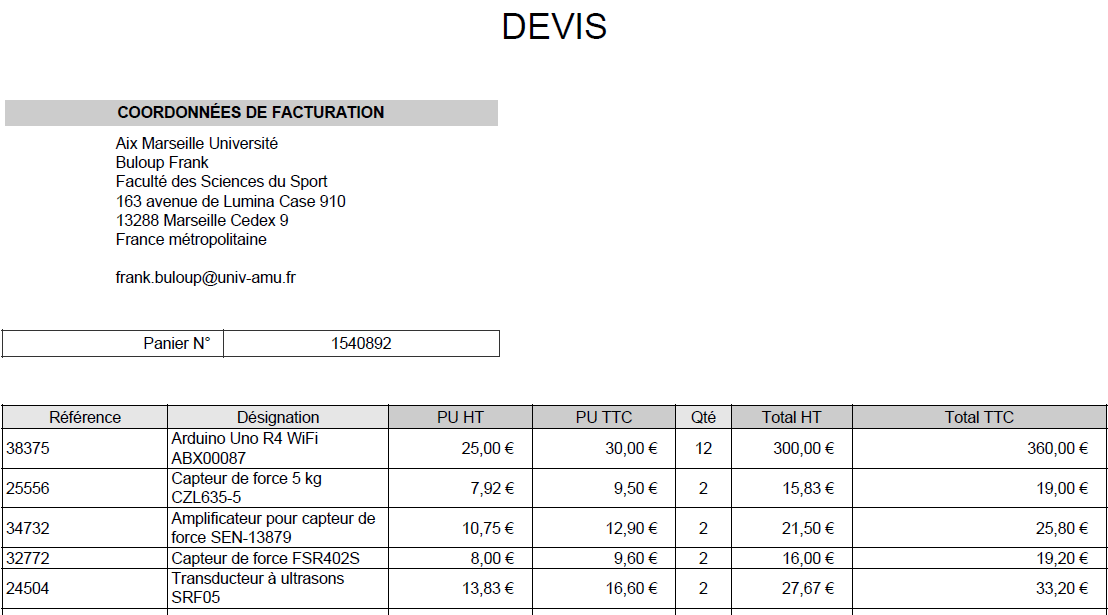
\includegraphics[scale=0.475]{images/devis.png}
\captionof{figure}{Exemple de devis - 10/09/2024}}

\end{frame}

\begin{frame}
	\center{
        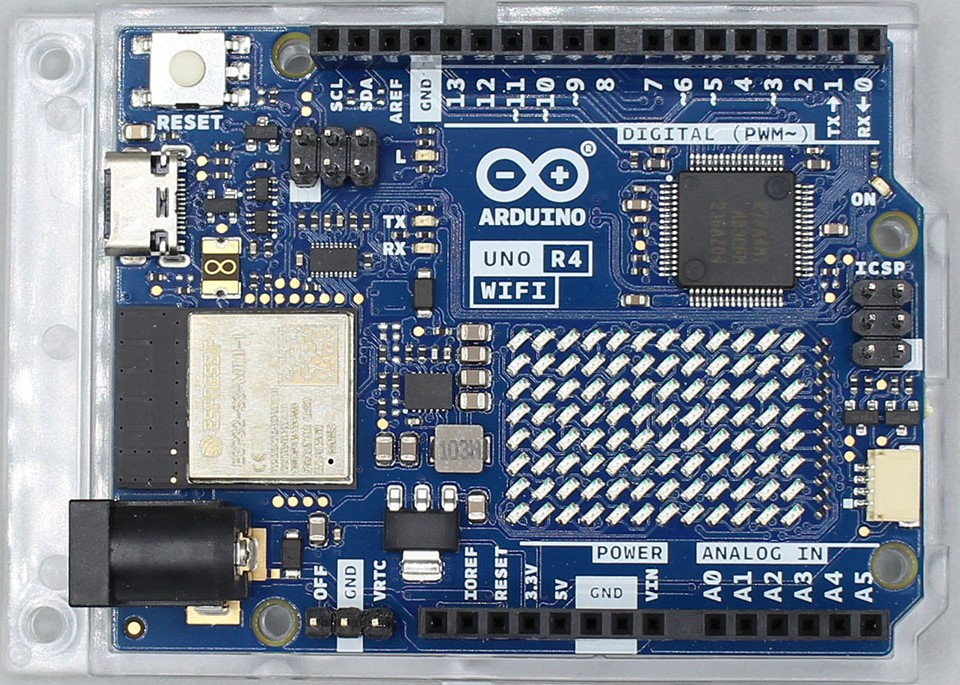
\includegraphics[scale=0.135]{images/ArduinoR4Wifi.jpg}
        \captionof{figure}{Arduino Uno R4 Wifi}}
        
        
\begin{block}{Projet global sur la base d'un Arduino Uno R4 Wifi}
\begin{itemize}
\item Création d'un gestionnaire d'essais en Python
\item Acquisition, visualisation et traitement des signaux
\item Répartir les taches dans l'équipe
\item Gérer les codes avec Git sur GitHub
\item Ne pas oublier de calibrer le capteur lorsque c'est nécessaire
\end{itemize}
\end{block}

\end{frame}

\begin{frame}
	\centering
        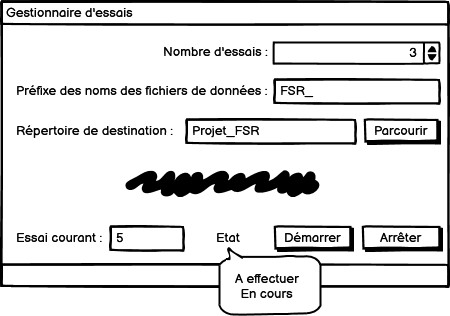
\includegraphics[scale=0.65]{images/GUI.png}
        \captionof{figure}{Exemple d'IHM du gestionnaire d'essais}
        
IHM : Interface Homme Machine (Graphical User Interface)
\end{frame}

\begin{frame}      
\begin{alertblock}{Conseils \& consignes !}
\begin{itemize}
\item Utilisez Arduino IDE pour programmer : port USB C
\item Utilisez ce même port pour communiquer avec l'arduino
\item Utilisez Python pour la partie PC (IHM avec Tkinter)
\item Utilisez la librairie pySerial de Python
\item Utilisez l'IDE de votre choix pour Python
\item Assurez-vous que le moniteur série (Arduino IDE) est fermé avant de lancer votre programme Python
\item Suivez les étapes ci-après : chaque étape est un commit
\item Le code générique pour un essai \textbf{doit} fonctionner \textbf{SANS} l'IHM
\item Le développement de l'IHM viendra dans un second temps
\item \textbf{\textcolor{red}{Chaque étape fera l'objet d'un commit sur GitHub}}
\end{itemize}
\end{alertblock}

\end{frame}

\section{Les étapes à suivre}
\begin{frame}
\begin{exampleblock}{GIT Step 1 - Synchronisation 1}
\begin{itemize}
\item Attendre la réception d'un caractère spécial pour démarrer la boucle loop() de l'Arduino
\item Ce step comportera également la configuration de la liaison série entre le PC et l'Arduino à 1Mbits/s, 8 bits de données, pas de parité et 1 bit de stop
\item Vous pourriez utiliser la LED interne (LED\_BUILTIN) pour vérifier que vous êtes bien entré dans la boucle
\end{itemize}
\end{exampleblock}
\begin{alertblock}{Universal Asynchronous Receiver/Transmitter}
\begin{itemize}
\item Point sur les UART/USART
\item SPI, I2C (TWI), 1-WIRE etc.

\centering
Pour plus d'infos : \textcolor{blue}{\textbf{\underline{\href{https://www.youtube.com/watch?v=ZdEVzz7TpLw}{Communication série et UART/USART}}}}
\end{itemize}
\end{alertblock}
\end{frame}

\begin{frame}
\begin{exampleblock}{GIT Step 2 - Synchronisation 2}
\begin{itemize}
\item Dans la boucle loop(), redémarrer l'Arduino dès réception d'un caractère spécial (Software reset)
\item Le redémarrage aura lieu après 10 secondes environ et sera initié côté PC
\end{itemize}
\end{exampleblock}
\begin{exampleblock}{GIT Step 3 - Comptage temporel}
\begin{itemize}
\item Mettre en place un système de comptage et de réinitialisation du temps en µs dans l'arduino
\item La réinitialisation aura lieu à chaque redémarrage de l'Arduino
\item Vous pourrez utiliser les fonctions Serial.println() et delay() pour vérifier votre code
\end{itemize}
\end{exampleblock}
\end{frame}

\begin{frame}
\begin{exampleblock}{GIT Step 4 - Transmission du comptage temporel}
\begin{itemize}
\item Transmettre ce comptage de temps de l'Arduino au PC
\item Vous utiliserez les fonctions sprintf() et Serial.println()
\item Supprimez les sorties consoles python qui prennent du temps
\item Supprimez les delay() côté Arduino si utilisés
\item Utilisez la commande flush du port série (Arduino et Python)
\item Vous accumulerez les valeurs temporelles dans un tableau times[] en secondes
\end{itemize}
\end{exampleblock}
\begin{exampleblock}{GIT Step 5 - Transmission valeurs du capteur}
\centering{\textbf{FSR (pour les deux postes) ou Potentiomètre}}
\begin{itemize}
\item Lire la valeur brute de la FSR ou du potentiomètre
\item Transmettre la valeur brute (SFR) ou calibrée (Potar) au PC
\item Vous utiliserez les mêmes fonctions sprintf() et Serial.println()
\end{itemize}
\end{exampleblock}
\end{frame}

\begin{frame}
\begin{exampleblock}{GIT Step 5 - Transmission valeurs du capteur}
\centering{\textbf{Jauge de contrainte (pour les deux postes)}}
\begin{itemize}
\item Calibrer la jauge avec les petites masses
\item Lire la valeur brute de la jauge
\item Transmettre la valeur calibrée au PC
\item Vous utiliserez les mêmes fonctions sprintf() et Serial.println()
\end{itemize}
\end{exampleblock}
\begin{exampleblock}{GIT Step 5 - Transmission valeurs du capteur}
\centering{\textbf{Capteur ultrason (pour les deux postes)}}
\begin{itemize}
\item Utiliser la librairie de \textcolor{blue}{\textbf{\underline{\href{https://github.com/RobTillaart/SRF05}{Rob Tillaard}}}}
\item Transmettre la valeur de distance en cm
\item Vous utiliserez les mêmes fonctions sprintf() et Serial.println()
\end{itemize}
\end{exampleblock}
\end{frame}

\begin{frame}
\begin{exampleblock}{GIT Step 5 - Transmission valeurs du capteur}
\centering{\textbf{Codeur Optique}}
\begin{itemize}
\item Utiliser le concept d'interruption pour réagir aux changements sur les entrées A et B du codeur
\item Dans les fonctions d'interruption, réinitialiser la valeur de l'angle si le signal Z du capteur est actif
\item Dans les fonctions d'interruption, utiliser les valeurs courantes et précédentes de A et B pour mettre à jour la valeur angulaire du capteur
\item Transmettre cette valeur au pc (dans la boucle loop())
\item Vous utiliserez les mêmes fonctions sprintf() et Serial.println()
\end{itemize}
\end{exampleblock}

\begin{alertblock}{Réagir à l'état d'une entrée : Polling (sondage) \& Interruption}
\centering
Pour plus d'infos : \textcolor{blue}{\textbf{\underline{\href{https://www.renesas.com/en/support/engineer-school/mcu-programming-peripherals-04-interrupts?srsltid=AfmBOoqWcjzACMZnxzxworQ_vp2hO_V4Mo23lAOhOzdPNzWOe2h45C7q}{Renesas - Interrupt}}}}
\end{alertblock}
\end{frame}

\begin{frame}
\begin{exampleblock}{GIT Step 6 - Accumulation, affichage et enregistrement des valeurs}
\begin{itemize}
\item Vous avez accumulé durant les dix secondes ces valeurs (signaux et temps) dans un tableau
\item Afficher le signal à la fin de ces dix secondes (graphe temporel)
\item Enregistrer les valeurs dans un fichier
\end{itemize}
\end{exampleblock}
\begin{exampleblock}{GIT Step 7 - Réaliser plusieurs essais}
\begin{itemize}
\item Ajouter une boucle pour réaliser plusieurs essais (e.g. 10 essais)
\item Prendre en compte le numéro d'essai dans le nom des fichiers de données
\end{itemize}
\end{exampleblock}
\begin{exampleblock}{GIT Step 8 - IHM}
\begin{itemize}
\item Ajouter une IHM permettant de paramétrer l'acquisition
\end{itemize}
\end{exampleblock}
\end{frame}

\begin{frame}
\begin{exampleblock}{GIT Steps suivants si possible}
\justifying
En vous appuyant sur les propositions ci-après, continuer en choisissant de vous répartir le travail de développement et de gestion de code en autonomie.
\end{exampleblock}
\end{frame}


\section{Pour aller plus loin sur les différents postes}
\subsection{Jauge de contrainte - 2 postes}
\begin{frame}
	\center{
        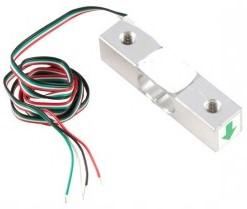
\includegraphics[scale=0.5]{images/czl635.jpg}
        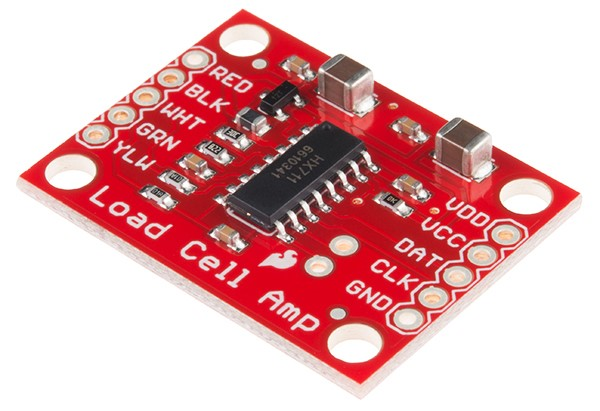
\includegraphics[scale=0.25]{images/AmpliJauge.jpg}
        \captionof{figure}{La jauge (CZL635-5) et son ampli (SEN-13879)}}	
	\begin{block}{TODO en plus ! (si possible ?)}
		\begin{itemize}
		\justifying
			\item Faire défiler la valeur de la masse sur la matrice LEDs de l'Arduino
			\item Afficher la valeur de la masse sur une page Web en utilisant le Wifi de l'arduino et un point d'accès mobile sur votre ordi ou téléphone
		\end{itemize}
	\end{block}
\end{frame}


\subsection{Résistance à détection de force - Temps de réponse}
\begin{frame}
\center{
        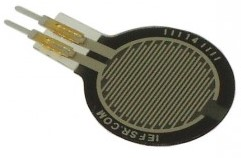
\includegraphics[scale=0.5]{images/fsr402s.jpg}
        \captionof{figure}{La résistance à détection de force (FSR402S)}}

	\begin{block}{TODO en plus ! (si possible ?)}
		\begin{itemize}
		\justifying
			\item Générer un top aléatoires avec la DEL de l'Arduino dans un intervalle de temps de 1 à 9 secondes. Le top durera 1 seconde.
			\item Taper sur la FSR dès que le top est perçu
			\item Enregistrer ces deux signaux (DEL et FSR)
			\item Caractériser leur écart temporel
		\end{itemize}
	\end{block}
\end{frame}

\subsection{Résistance à détection de force - Comptage}
\begin{frame}
\center{
        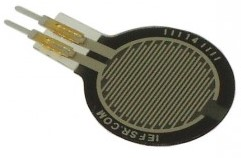
\includegraphics[scale=0.5]{images/fsr402s.jpg}
        \captionof{figure}{La résistance à détection de force (FSR402S)}}

	\begin{block}{TODO en plus ! (si possible ?)}
		\begin{itemize} 
		\justifying
			\item Taper sur la FSR régulièrement
			\item Compter le nombre de tapes
		\end{itemize}
	\end{block}
\end{frame}

\subsection{Capteur à ultrason - 2 postes}
\begin{frame}
\center{
        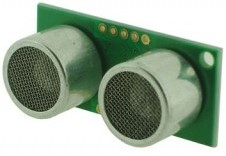
\includegraphics[scale=0.6]{images/SRF05.jpg}
        \captionof{figure}{Le capteur à ultrason (SRF05)}}
	\begin{block}{TODO en plus ! (si possible ?)}
		\begin{itemize}
		\justifying
			\item Faire défiler la valeur de la distance sur la matrice LEDs de l'Arduino
			\item Faire clignoter la LED de l'Arduino en liant la cadence de clignotement à la distance donnée par le capteur à ultrason 
		\end{itemize}
	\end{block}
\end{frame}

\subsection{Potentiomètre - Pendule simple*}
\begin{frame}
	\center{
        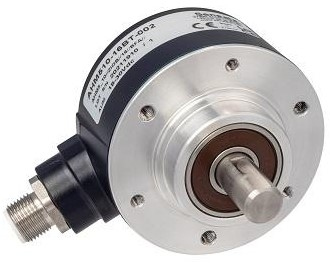
\includegraphics[scale=0.6]{images/ahm5.jpg}
        \captionof{figure}{Le potentiomètre (AHM5)}}
	\begin{block}{TODO en plus ! (si possible ?)}
		\begin{itemize}
		\justifying
			\item Enregistrer pour plusieurs positions de la masse
			\item Estimer la longueur du bras d'oscillation pour chaque position
			\item Identifier un système qui simule le mouvement
		\end{itemize}
	\end{block}
\end{frame}

\subsection{Codeur optique*}
\begin{frame}
\center{
        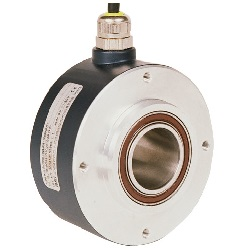
\includegraphics[scale=1.5]{images/codeur.jpg}
        \captionof{figure}{Le codeur optique}}
	\begin{block}{TODO en plus ! (si possible ?) Retrogaming Pong ;-)}
		\begin{itemize}
		\justifying
			\item Positionner une raquette du jeu en fonction de la valeur envoyée par le codeur
		\end{itemize}
	\end{block}
\end{frame}



\end{document}
